\documentclass[11pt]{article}
\usepackage[utf8]{inputenc}
\usepackage[T1]{fontenc}
\usepackage[margin = 2cm]{geometry}

\usepackage{palatino}
\usepackage{amsmath}
\usepackage{graphicx}
\usepackage{listings}
\usepackage{mathpazo}
\usepackage{hyperref}
\usepackage{courier}
\usepackage{subfigure}

\lstset{basicstyle=\normalsize\ttfamily, breaklines=true}

\author{Samuele Bosi, Marco Ferrè, Philip Michael Grasselli, Simone Mariani}
\title{\textbf{CMLS Homework 3 – Voice Harmonizer}}
\date{\today}

\begin{document}
\maketitle
\tableofcontents

\section{Introduction}
In this third and last assignment, our task was to create a \textbf{voice harmonizer}, both the effect and the mobile control interface, plus another couple of effects (tremolo and reverb). We used \textbf{SuperCollider} to implement the former, and \textbf{TouchOSC} for the latter: a voice coming from any microphone connected to the computer could pass across this system.\\
For the repository, this is the URL for GitHub: \url{https://github.com/marcoferre/CMLS-HW3}.

\section{A Glance of Harmonics}

The choice of the number and the interval between notes was not as straightforward as we thought at the beginning, since the effect has to be realistic. The simplest idea was to consider only octaves, as it is typical of almost all instruments, and this is evident whilst applying the Fourier Transform of a sound excerpt of a note played by an instrument.\\
To give a \textit{minor} or \textit{major} harmonization, the minor and the major \textbf{third interval} was taken into consideration, as the musical theory clearly explains.

\section{The Harmonizer}

As previously touched upon, the voice harmonizer is composed by two parts: the SuperCollider algorithm and the TouchOSC GUI for touch devices.

\subsection{The SuperCollider Code}

After booting the \texttt{localhost} server with the \texttt{s.boot} line, we define the arguments related to the knobs of the several effects inside the pad: the pitch shift, the array referred to the harmonics, the room effect for the reverberation, the X and Y coordinates for the tremolo (frequency and amplitude), and the attack.\\

The sound is captured from the microphone through the command line:

\begin{verbatim}
in = Mix.new(SoundIn.ar([0,1]));
\end{verbatim}

It follows that the amplitude is being deemed by the \texttt{Amplitude} class for each sample, and its value brought to the \texttt{amp} variable.\\

We, then, define the number of harmonics by setting up the array of partials:
\begin{itemize}
\item if we're moving by octaves, we just divide or multiply by $2^k$, with $k\in\mathbb{Z}$:
\item if we're considering also the minor thirds, we add a $\sqrt[3]{2}$ correction factor;
\item if major thirds are needed, we place a $\sqrt[4]{2}$ correction factor.
\end{itemize}
All the seven harmonics are naturally stored into the same number of variables \texttt{v1}, \texttt{v2}, etc.

\subsubsection{The \texttt{PitchShift} Class}
The frequency translation occurs thanks to the \texttt{PitchShift} class: several parameters could be set, including:
\begin{itemize}
\item the \textbf{width} of the frame applied to the input signal;
\item the \textbf{translation rate} of the harmonics with respect to the fundamental frequency;
\item the frequency \textbf{ripple} of the harmonics;
\item the temporal \textbf{delay} of the harmonics;
\item the \textbf{amplitude} of the output signal. Attack and release values are picked up by the previously declared \texttt{amp} variable.
\end{itemize}

\subsubsection{Reverberation}

\begin{figure}
\centering
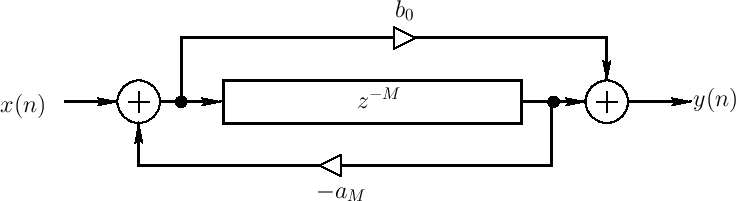
\includegraphics[width=0.5\textwidth]{Allpass.png}
\label{fig:AllpassFilter}
\caption{The Schröder all-pass filter}
\end{figure}

The class \texttt{FreeVerb} lets you design the reverberation effect, in which you can set up a couple of parameters: the dry/wet level and the room effect. This was our choice, since it was simpler and very effective.\\
Another way to build this spatial effect could be to implement a \textbf{Schröder all-pass filter}, which is shown on figure \ref{fig:AllpassFilter}, and it's transfer function is:
\begin{equation}
\displaystyle
H(z)=\frac{b_0+z^{-M}}{1-a_M z^{-M}}
\end{equation}
where $b_0 = a^*_M$, to let it become a real all-pass filter. In SuperCollider, the class \texttt{AllPassN} implements this function.

\subsection{The GUI}
\begin{figure}
\centering
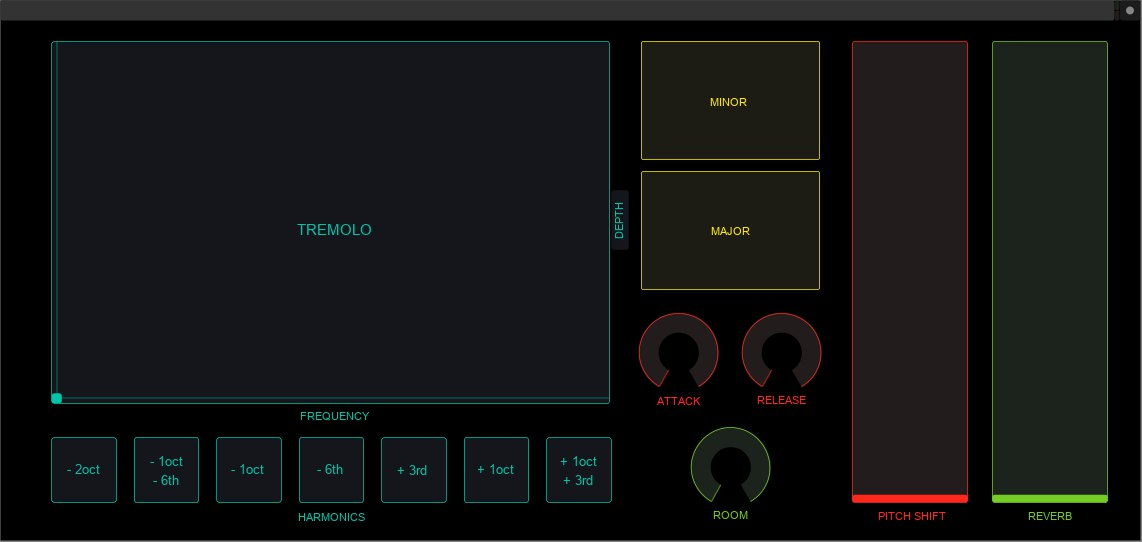
\includegraphics[width=1\textwidth]{SynthesizerOSC.jpg}
\caption{The Graphical User Interface of the Voice Harmonizer in its final version}
\label{fig:TouchOSC}
\end{figure}

The software \textbf{TouchOSC} was used for the visual part of our synthesizer, and it's shown in Figure \ref{fig:TouchOSC}.\\

The controller receives the harmonizer messages of \texttt{pitchFollow1}, and we declare two variables related to the input and the output signal addresses. Once completed these first tweaks, we proceed to define the default values for all the buttons, in order to initialize the GUI.\\
All the \texttt{OSCdef} associated to all controls are very similar and straightforward in their functionality, as they receive and send messages to the SuperCollider's post window. One last thing related to this interface is that major and minor buttons are mutually exclusive.

\section{What's Next?}
A possible implementation of our commitment could be -- in a hardware fashion -- to transfer this interface to a Raspberry-controlled pedal board; by using a LCD display we could manage the currently applied settings, and by using an expression pedal and foot-switches we could control all the other available effects. All this stuff may be useful in case of live performances.

\end{document}